\documentclass[border=8pt]{standalone}
\usepackage{fontspec}
\usepackage{tikz}
\usetikzlibrary{calc}
\definecolor{navy}{HTML}{203A93}
\definecolor{uniongreen}{HTML}{A9E6C3}
\definecolor{intersectionpurple}{HTML}{B58BC7}
\definecolor{differenceblue}{HTML}{BFDDF2}
\begin{document}
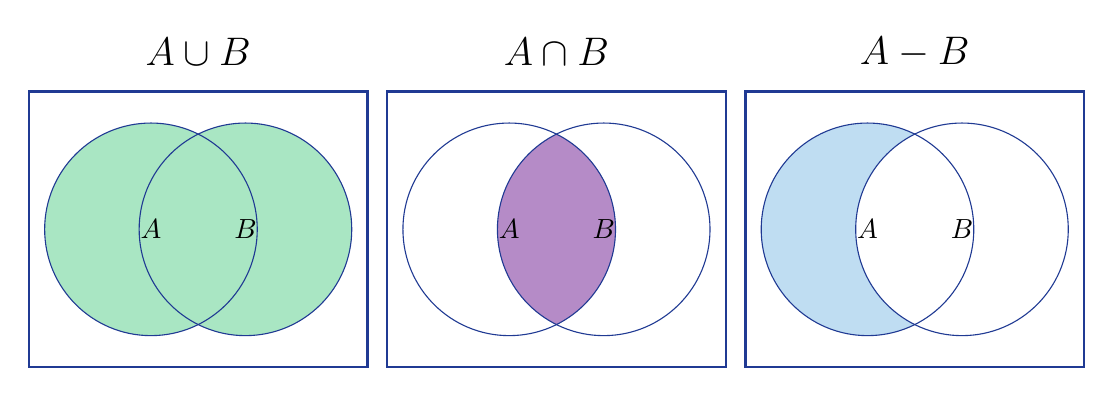
\begin{tikzpicture}[font=\itshape]
  \def\r{1.35}
  \def\d{0.82}
  \newcommand{\panel}[1]{\draw[navy,line width=.9pt] (#1-2.15,-1.75) rectangle (#1+2.15,1.75);}
  % Union: one uniform shade over A union B.
  \node[font=\Large] at (-4.55,2.25) {$A\cup B$};
  \panel{-4.55}
  \coordinate (a1) at (-5.15,0); \coordinate (b1) at (-3.95,0);
  \fill[uniongreen] (a1) circle (\r) (b1) circle (\r);
  \draw[navy] (a1) circle (\r); \draw[navy] (b1) circle (\r);
  \node at (-5.15,0) {$A$}; \node at (-3.95,0) {$B$};
  % Intersection: only the lens shaded.
  \node[font=\Large] at (0,2.25) {$A\cap B$};
  \panel{0}
  \coordinate (a2) at (-.6,0); \coordinate (b2) at (.6,0);
  \begin{scope}\clip (a2) circle (\r); \fill[intersectionpurple] (b2) circle (\r);\end{scope}
  \draw[navy] (a2) circle (\r); \draw[navy] (b2) circle (\r);
  \node at (-.6,0) {$A$}; \node at (.6,0) {$B$};
  % Difference: only A outside B shaded.
  \node[font=\Large] at (4.55,2.25) {$A-B$};
  \panel{4.55}
  \coordinate (a3) at (3.95,0); \coordinate (b3) at (5.15,0);
  \fill[differenceblue] (a3) circle (\r);
  \begin{scope}\clip (a3) circle (\r); \fill[white] (b3) circle (\r);\end{scope}
  \draw[navy] (a3) circle (\r); \draw[navy] (b3) circle (\r);
  \node at (3.95,0) {$A$}; \node at (5.15,0) {$B$};
\end{tikzpicture}
\end{document}
